\documentclass[a4paper, 12pt, twoside]{article}
\usepackage[utf8]{inputenc}		% LaTeX, comprend les accents !
\usepackage[T1]{fontenc}		
\usepackage[francais]{babel}
\usepackage{lmodern}
\usepackage{ae,aecompl}
\usepackage[top=2.5cm, bottom=2cm, 
			left=3cm, right=2.5cm,
			headheight=15pt]{geometry}
\usepackage{graphicx}
\usepackage{eso-pic}	
\usepackage{array}	
\makeatletter
\def\@ecole{école}
\newcommand{\ecole}[1]{
  \def\@ecole{#1}
}
\def\@domaine{}
\newcommand{\domaine}[1]{
  \def\@domaine{#1}
}

\def\@specialite{Spécialité}
\newcommand{\specialite}[1]{
  \def\@specialite{#1}
}


\def\@master{Master}
\newcommand{\master}[1]{
  \def\@master{#1}
}

\def\@adresse{Adresse}
\newcommand{\adresse}[1]{
  \def\@adresse{#1}
}

\def\@encadranta{}
\newcommand{\encadranta}[1]{
  \def\@encadranta{#1}
}

\def\@encadrantb{}
\newcommand{\encadrantb}[1]{
  \def\@encadrantb{#1}
}
\def\@auteura{}{}{}
\newcommand{\auteura}[1]{
  \def\@auteura{#1}
}
\def\@auteurb{}{}{}
\newcommand{\auteurb}[1]{
  \def\@auteurb{#1}
}
\def\@auteurc{}{}{}
\newcommand{\auteurc}[1]{
  \def\@auteurc{#1}
}
\def\@auteurd{}{}{}
\newcommand{\auteurd}[1]{
  \def\@auteurd{#1}
}
\makeatother




\makeatletter
\newcommand{\pagedegarde}{
\newgeometry{top=2.5cm, bottom=1cm, left=2cm, right=1cm}
  \begin{titlepage}
  \centering
      
\includegraphics[width=1\textwidth]{limogelogo.pdf}
    \vspace{1cm}
      {\huge 
    \vspace{0.5cm}
        {\huge\bfseries \@ecole}\\
    \vspace{0.2cm}
        {\Large\bfseries \@domaine}\\
    \vspace{0.5cm}
        {\Large\bfseries Master 1 }\\
    \vspace{0.2cm}
        {\large\bfseries Sécurité informatique et cryptologie }\\
    \vspace{1cm}
    	MEMOIRE DU SECOND SEMESTRE}\\
    \vfill
       {\LARGE \color[rgb]{0,0,1} \bfseries{\@title}} \\
    \vspace{2cm}
    	{\bfseries \@auteura}\\
    	{\bfseries \@auteurb}\\
    	{\bfseries \@auteurc}\\
    	{\bfseries \@auteurd}\\
    \vspace{0.5cm}
        Encadrants :\\
        {\bfseries \@encadranta}\\
        {\bfseries \@encadrantb}\\
    \vspace{0.5cm}
        {\Large\bfseries \@date}\\
    \vfill
  \end{titlepage}
\restoregeometry
}
\author{}
\auteura{Thanina \textsc{Alili}}
\auteurb{Thibault \textsc{Debonnière}}
\auteurc{Baptiste \textsc{Decrand}}
\auteurd{Ndiasse \textsc{Thioune}}
\title{Analyse Forensic d'un Ransomware}
\master{Master 1 Informatique}
\specialite{CRYPTIS}
\encadranta{Jean-Louis \textsc{Lanet}}
\encadrantb{Benoit \textsc{Crepin}}
\date{Novembre 2017}
\ecole{UNIVERSIT\'{E} DE LIMOGES}
\domaine{
	\textbf{FACULT\'{E} DES SCIENCES ET TECHNIQUES}
}
\begin{document}
\pagedegarde
\tableofcontents
\section{Introduction}
\subsection{Contexte}
Cette application est lié au mémoire de la première année de Master Informatique à l'université de Limoges. Le sujet du mémoire étant "Analyse forensic d'un Ransomware", cette application à pour objectif de déduire la classe d'un ransomware depuis une capture de mémoire vive d'un système infecté.

\subsection{Intérêts du document}
Ce document a pour but d'indiquer l'architecture et les choix techniques de l'application au développeur. Il indique ainsi toutes les informations nécessaires à la conception et au développement du programme. 

\subsection{Présentation de l'application}
L'application permettre à l'utilisateur de soumettre ces captures de mémoires à l'analyse, celle-ci lui renverra les taux de ressemblance de sa capture avec les différentes classes de ransomwares.
L'application est développé en langage Java.

\section{Description de l'application}
\subsection{Objectifs}
L'objectif de l'application est de permettre à l'utilisateur de pouvoir analyser au mieux les captures mémoires de ransomwares afin que celui-ci puisse en déduire facilement à quelles familles ils appartiennent. Pour cela, l'utilisateur aura accès à huit métriques différentes qui lui donneront huit différentes formes de rapprochements avec les classes de ransomwares.

Lors du lancement du programme, l'utilisateur indiquera le chemin 
du fichier à analyser et sélectionnera les métriques à utiliser.

Une fois l'analyse lancé, les résultats s'afficheront sous forme de tableau avec pour chaque métriques et classes de ransomware le rapprochement calculé.

\subsection{Architecture global de l'application}
L'architecture global de l'application se base sur un modèle standard MVC (Modèle vue Contrôleur) de développement d'application et d'interface graphique.
\begin{figure}[!h]
\centering
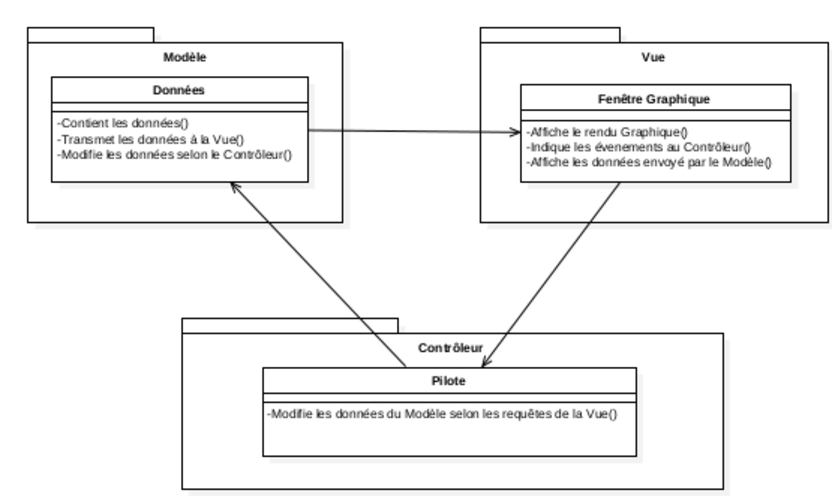
\includegraphics{MVC.pdf}
\caption{Modèle MVC}
\end{figure}

\section{Conception}
\subsection{Architecture interne}


\subsection{Algorithmes}

\section{Spécification des Données Persistantes}
\subsection{Données des classes de Ransomware}

\section{Spécification IHM}
\subsection{Schéma de Navigation}

Notre outil est extrêmement simpliste d'utilisation  :
\begin{figure}[!h]
\centering
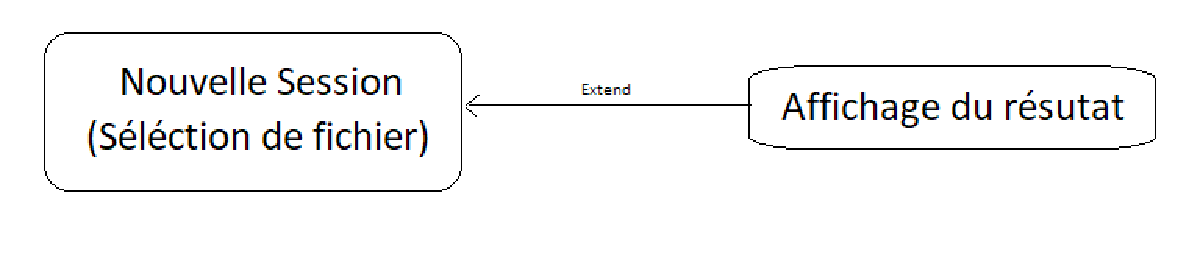
\includegraphics[scale=0.75]{utilisation.pdf}
\caption{}
\end{figure}






\newpage
\subsection{Maquettes et Interface}
\begin{figure}[!h]
\centering
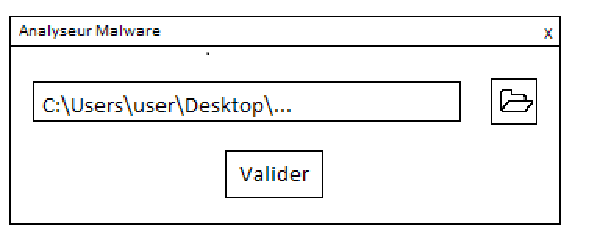
\includegraphics{maquette1.pdf}
\caption{}
\end{figure}
\begin{figure}[!h]
\centering
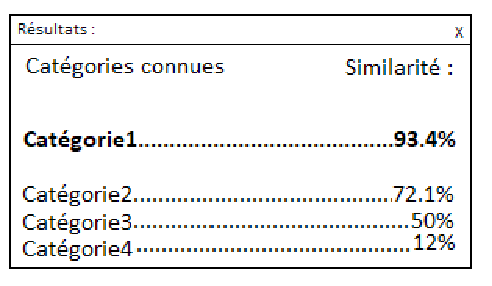
\includegraphics{maquette2.pdf}
\caption{}
\end{figure}


L'interface utilisateur du programme se voudra relativement simpliste, le but de celle-ci sera avant tout d'être fonctionnelle plus que visuelle. 
Elle disposera d'une zone de saisie pour le chemin du fichier de capture qui sera l'entrée de notre programme, ainsi qu'un simple bouton pour lancer le balayage parmi la base de données(Figure2).

~\par
Une fois le balayage effectuée, une fenêtre s'ouvrira affichant le pourcentage de similarité entre l'entrée et les catégories les plus probable(Figure3). 
Autre possibilité : un bouton permettant d'afficher la base de données collectées jusqu'à présent par le programme.

\end{document}